\documentclass[main.tex]{subfiles}

\begin{document}

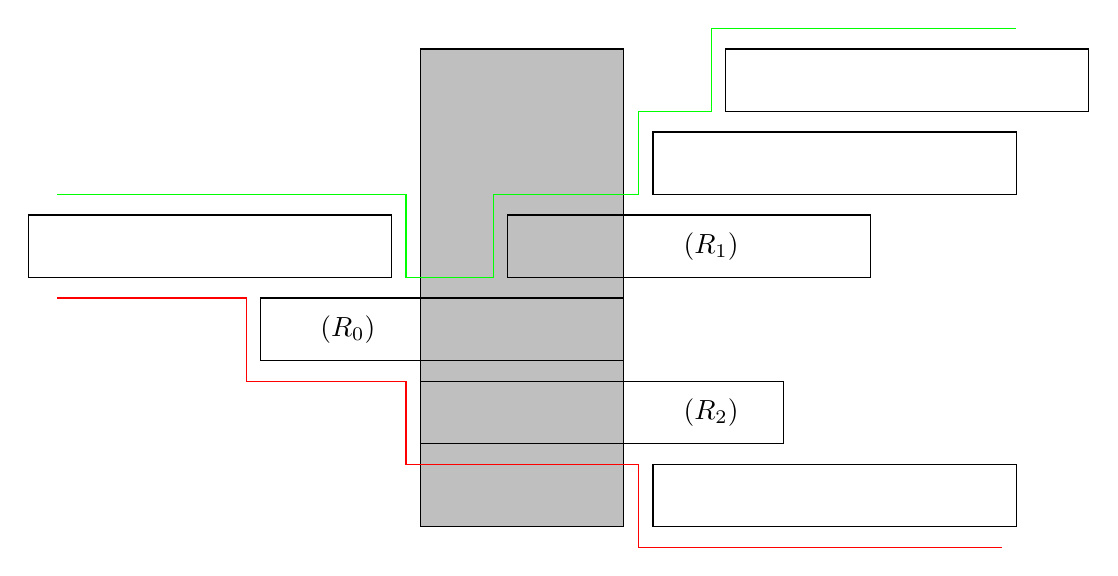
\begin{tikzpicture}[x=0.75pt,y=0.75pt,yscale=-1,xscale=0.7]

% Reads
\draw   (0,   80) -- (250, 80) -- (250,110) -- (0,  110) -- cycle ;
\draw   (160,120) -- (410,120) -- (410,150) -- (160,150) -- cycle ;
\draw   (270,160) -- (520,160) -- (520,190) -- (270,190) -- cycle ;
\draw   (330, 80) -- (580, 80) -- (580,110) -- (330,110) -- cycle ;
\draw   (430,200) -- (680,200) -- (680,230) -- (430,230) -- cycle ;
\draw   (430, 40) -- (680, 40) -- (680, 70) -- (430, 70) -- cycle ;
\draw   (480,  0) -- (730,  0) -- (730, 30) -- (480, 30) -- cycle ;

% Repetition region
\draw [fill={rgb, 255:red, 0; green, 0; blue, 0 }, fill opacity=0.25] (270,0) -- (410,0) -- (410,230) -- (270,230) -- cycle;

% Two path repetition
\draw [color={rgb, 255:red, 255; green, 0; blue, 0 }, draw opacity=1] (20, 120) -- ++ (130, 0) -- ++ (0, 40) -- ++ (110, 0) -- ++ (0, 40) -- ++ (160, 0) -- ++ (0, 40) -- ++ (250, 0);

\draw [color={rgb, 255:red, 0; green, 255; blue, 0 }  ,draw opacity=1 ]   (20, 70) -- ++ (240, 0) -- ++ (0, 40) -- ++ (60, 0) -- ++ (0, -40) -- ++ (100, 0) -- ++ (0, -40) -- ++ (50, 0) -- ++ (0, -40) -- ++ (210, 0);

\draw (220,135) node  [align=left] {($R_0$)};
\draw (470,95) node  [align=left] {($R_1$)};
\draw (470,175) node  [align=left] {($R_2$)};

\end{tikzpicture}
\end{document}
